Der Bereich der qualitativen Sichtprüfung hat grundlegend die Aufgabe, spiegelnde Oberflächen nach bestimmten Kriterien in gut und fehlerhaft zu unterteilen.
Die Aufbauten für solche Verfahren sehen in der Regel ähnlich aus wie auch in Abbildung \ref{img:aufbau}.
Zur Analyse dieser spiegelnden Oberflächen ist es nicht unbedingt nötig, ein dreidimensionales Oberflächenmodell zu erzeugen.
Ein wesentlicher Unterschied ist deshalb, dass die Informationen über den Systemaufbau nicht zwingend notwendig für Berechnungen sind.
Um eine möglichst allgemein einsetzbare Lösung zu entwickeln, ist dies ein essenzieller Vorteil.
Die Vorgehensweise bei diesen Verfahren basiert in den meisten Fällen darauf, die Abweichungen der Oberflächenstruktur zu einem Referenzobjekt zu bewerten.
Abhängig von den einzelnen Oberflächenmerkmalen können verschiedene Muster und Strategien zur Auswertung eingesetzt werden.

\p
In seiner Dissertation \glqq Deflektometrie zur automatischen Sichtprüfung und Rekonstruktion spiegelnder Oberflächen\grqq ~\cite{kit_werling} listet Stefan Bruno Werling vom Karlsruher Institut für Technologie einige Auswertungsmöglichkeiten auf.
Daraus sind die Folgenden eine Auswahl seiner Strategien:

\begin{itemize}
	\item Untersucht man auf der Oberfläche eines Objekts ein sinusförmiges Streifenmuster, dann können im Frequenzraum Abweichungen des Musters von einem \glqq Idealmuster\grqq ~bzw. Referenzmuster festgestellt werden.
	Dadurch entdeckt man Unterschiede in der Oberflächenkrüm\-mung.
	Die Transformation des Bildes in den Frequenzraum wird durch die Fourier-Transformation erreicht.
	
	\item Nutzt man zur Auswertung ein Schachbrettmuster, so können durch die Wahl eines geeigneten Schwellwerts bestimmte Flächen segmentiert und geometrisch analysiert werden.
	Nach der Analyse sollen Anomalien der geometrischen Merkmale Aussagen über die Krümmung treffen.
	
	\item Besonders kleine Fehler und Defekte der Oberflächenstruktur lassen sich an Hell-Dunkelübergängen gut hervorheben.
	Hierfür kann man einfache Streifenmuster analysieren, wie es in Abbildung \ref{img:scratch} gezeigt ist.
	Dieses Verfahren wird im Kapitel \ref{chp:sichtpruefungDurchLichtstreuung} näher beschrieben.
\end{itemize}

\begin{figure}[H]
	\centering
	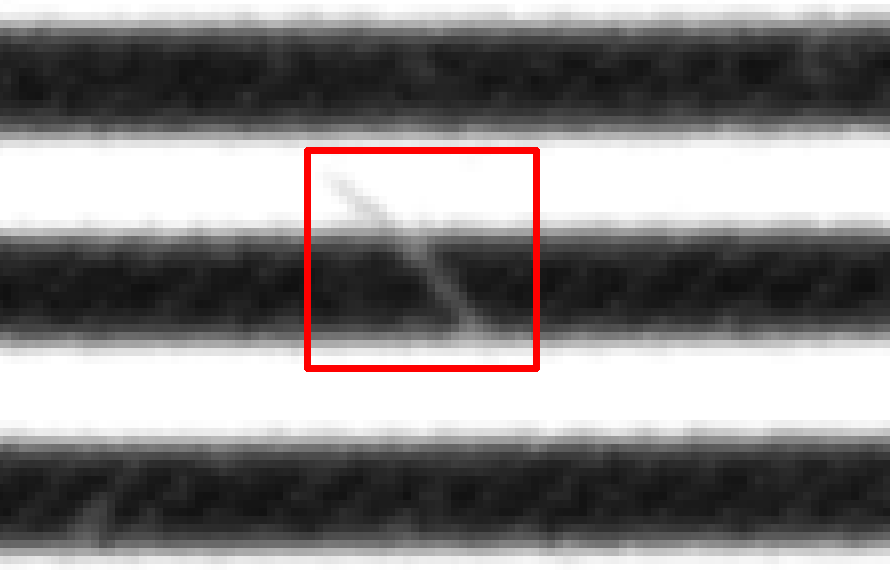
\includegraphics[width=0.5\textwidth]{02_grundlagenDerDeflektometrie/qualitativeSichtpruefung/figures/scratch}
	\caption[Kratzer an Hell-Dunkel-Übergang eines Streifenmusters]{Kratzer an Hell-Dunkel-Übergang eines Streifenmusters}
	\label{img:scratch}
\end{figure}

\noindent
Neben diesen Verfahren gibt es auch noch die Möglichkeit die Krümmung zu analysieren, indem man die Zuordnung zwischen Kamera- und Bildschirmkoordinaten (siehe Abschnitt \ref{sec:rekonstruktion}) auswertet.
Analytisch betrachtet ändert sich bei starken Krümmungen der Oberfläche auch die Oberflächennormale an der lokalen Stelle besonders stark.
Mit dem Reflexionsgesetz wird damit deutlich, dass lokal in der Reflexion große Abweichungen von einer ebenen Spiegelung auftreten.
Das lässt sich in der beschriebenen Zuordnung direkt erkennen, ohne weitere Systemparameter berücksichtigen zu müssen.
Dies wird im Abschnitt \ref{sec:auswertungDeflektometrischeRegistrierung} genauer behandelt.

\p
Durch die Variabilität der Deflektometrie und der vielen Möglichkeiten der qualitativen Sichtprüfung lassen sich z. B. durch Veränderung bestimmter Muster zahlreiche verschiedene Verfahren aufstellen, um eine Objektoberfläche zu analysieren.
Aus dem Grund wird keine allgemeine Funktionsweise von deflektometrischen Verfahren für die qualitative Sichtprüfung beschrieben, sondern auf konkrete Verfahren (vgl. Kapitel \ref{chp:sichtpruefungDurchLichtstreuung}) eingegangen.